%! Author = Saeid Yazdani
%! Date = 9/6/2024

\section{Software Components}
\label{software-components}

The main overview of the software in the system has already been presented
in \autoref{ch:proposed-control-loop} as a prerequisite to
realization of the hardware (\autoref{ch:hardware-realization}).
Therefore, this chapter looks into the actual implementation of the software
components.

\autoref{fig:software-components-overview} shows the three main components that
work in tandem to operate the system:

The \textbf{Operator Software} (\acs{GUI} or \acs{API})
serves as the bridge between the user and the \acs{HVS} system for
setting desired output values, debugging the system internals, etc.
The operator is required to provide the initial configuration of the system
including calibration data and if available, customized compensation settings
for a given \acs{DUT}.

The \textbf{Microcontroller Software} is responsible for
managing communication with the operator through the messaging engine and
perform system management by handling relays and sensors.
The \acs{MCU} is responsible for transferring data such as configuration and compensation
data, measurement data and actual status between the FPGA and the operator
software through the implemented Avalon bus.

The \textbf{FPGA Software} is dedicated to the real-time processing of internal
signals of the system between frontend and
amplifier boards using the provisioned \acs{ADC}s and \acs{DAC}s.
The control algorithm implements the logic for comparison of input
and output with setpoint, performs error calculations and issues
new signals to the driver stage to stay near the setpoint.


\begin{figure}[b!]
    \centering
    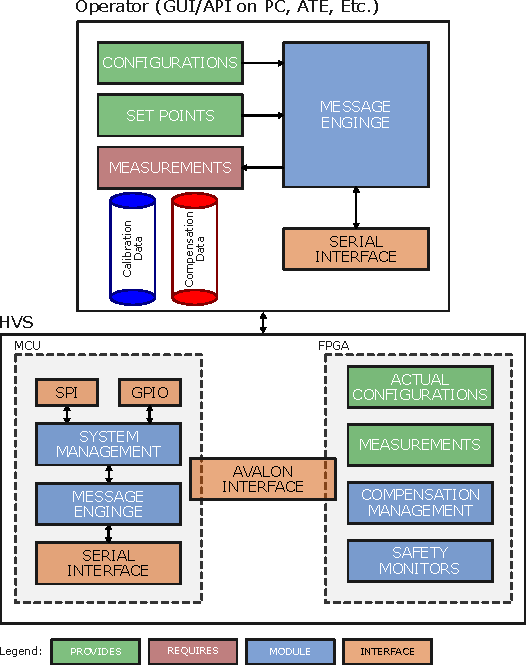
\includegraphics[width=0.8\textwidth]
    {figures/software/software-overview}
    \caption[Overview of the Software Components]{
        Overview of the software components that operate the system.
    }
    \label{fig:software-components-overview}
\end{figure}
